\documentclass{article}
\usepackage[utf8]{inputenc}
\usepackage{amsmath}
\usepackage{tcolorbox}
\usepackage{amssymb}
\usepackage{amsthm}
\theoremstyle{definition}
\newtheorem{example}{Example}[section]


\usepackage[
top    = 2.50cm,
bottom = 2.50cm,
left   = 2.75cm,
right  = 2.75cm]{geometry}
\usepackage{fancyhdr}
\pagestyle{fancy}
\lhead{Advanced computation}
\rhead{EPFL/Alp Ozen}


\newtheorem{thm}{Theorem}


\title{Advanced Computation}
\author{alp.ozen}
\date{\vspace{-5ex}}
\newtheorem{theorem}{Theorem}[section]

\begin{document}

\maketitle
\section{Propositional logic }
\subsection{Propositions}
A proposition is a declarative sentence that is either true or false. 
\begin{tcolorbox}
How much does it cost? \textbf{is not a proposition}
\\
I like red \textbf{is a proposition}
\end{tcolorbox}

To make life easier, we represent propositional statements through letters such as $p$. 
\\

The conditional statement $p\implies q$ appears very often. Thus, we have the \textit{converse,contrapositive and inverse} which are:
\\
\textbf{converse}: $q \implies p$
\\
\textbf{contrapositive}: $ \neg q \implies \neg p $
\\
\textbf{inverse}: $ \neg p \implies \neg q$
\\

We note that a conditional is logically equivalent to its contrapositive. 

\begin{tcolorbox}
\centering
\begin{array}{cccccc}
 p & q & p $\implies$ q & \neg q & \neg p & \neg q $\implies$ \neg p \\
 \hline
t & t & t & f & f & t\\
t & f & f & t & f & f\\
f & t & t & f & t & t\\
f & f & t & t & t & t
\end{array}
\end{tcolorbox}

\subsection{Precedence of logical operators}

\begin{figure}[h]
    \centering
    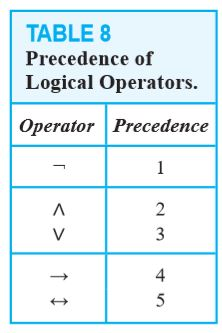
\includegraphics{figures/precedence}
\end{figure}


%below are notes from lecture one 








\end{document}